\chapter{Тригонометрия}\label{chap:c15}\markright{Глава 24}
\begin{definition}\term{Радиан} (\emph{radian}) — единица измерения угла. Угол в \(1\) радиан — центральный угол, которому соответствует дуга длины, равной радиусу окружности. Радианная мера центрального угла равна \(\alpha=\frac{l}{r}\), где \(l\) — длина дуги, \(r>0\) — радиус. Полный оборот: \(2\pi\) радиан, то есть \(360^\circ\).\end{definition}
Положительные углы отсчитывают от точки \((1;0)\) единичной окружности против часовой стрелки, отрицательные — по часовой.
\begin{definition}\term{Косинус} (\emph{cosine}) \(\cos\alpha\) — горизонтальная координата точки единичной окружности, полученной поворотом точки \((1;0)\) на угол \(\alpha\).\end{definition}
\begin{definition}\term{Синус} (\emph{sine}) \(\sin\alpha\) — вертикальная координата точки единичной окружности, полученной поворотом точки \((1;0)\) на угол \(\alpha\).\end{definition}
\begin{definition}\term{Тангенс} (\emph{tangent}): \(\operatorname{tg}  \alpha  = \frac{\sin  \alpha }{\cos  \alpha }\) при \(\cos  \alpha  \ne  0\).\end{definition}
\begin{definition}\term{Период функции} (\emph{period of a function}) — ненулевое число \(T\), при сдвиге аргумента на которое область определения сохраняется и \(f (x + T) = f (x)\).\end{definition}
\section{Основные тождества и свойства}
\par\addvspace{5pt}\begin{lrbox}{\CatFlowBox}\begin{minipage}[t]{\linewidth}
\setlength{\parskip}{5pt}\setlength{\columnsep}{4.5mm}\setlength{\intextsep}{0pt}
\begin{wrapfigure}[12]{r}{54mm}
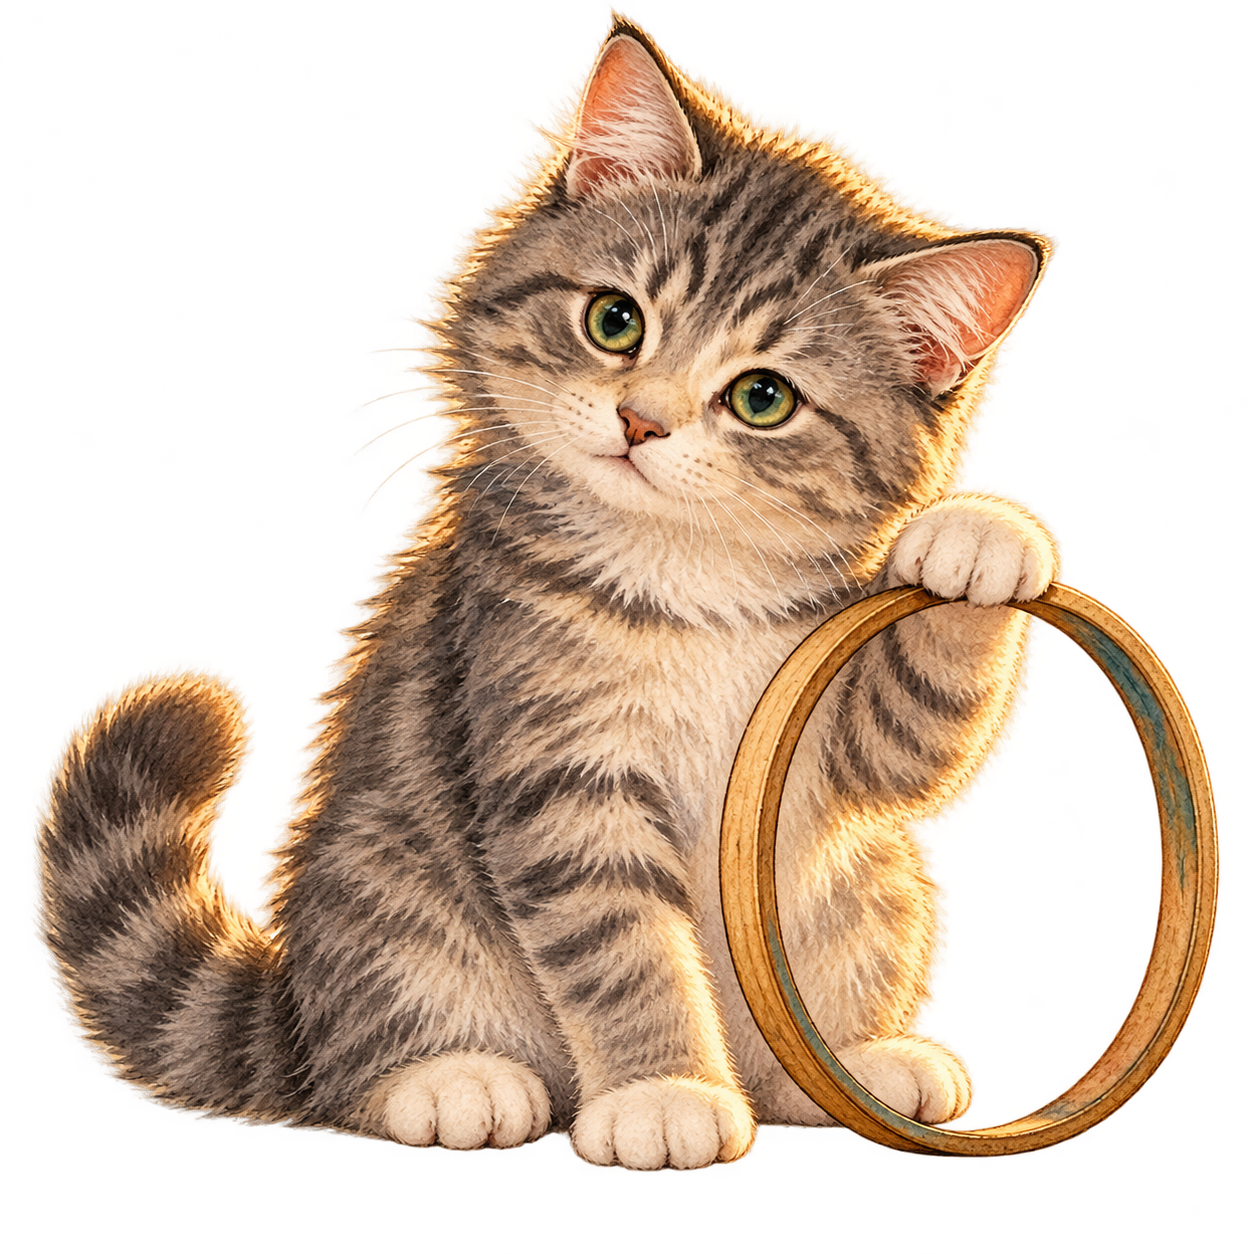
\includegraphics[width=54mm,height=58mm,keepaspectratio]{images/unique/art-26.png}
\label{catflow:26}
\end{wrapfigure}
\(\sin ^{2} \alpha  + \cos ^{2} \alpha  = 1\). Значения синуса и косинуса лежат в \([- 1;\allowbreak 1]\).\par
\(\sin  (- \alpha ) = - \sin  \alpha ;\allowbreak \cos  (- \alpha ) = \cos  \alpha \).\par
\(\sin  (\pi  - \alpha ) = \sin  \alpha ;\allowbreak \cos  (\pi  - \alpha ) = - \cos  \alpha \).\par
Наименьший положительный период синуса и косинуса равен \(2 \pi \). Для \(\sin  (kx)\) и \(\cos  (kx)\) при \(k \ne  0\) он равен \(\frac{2 \pi }{| k |}\).\par
\par\WFclear\end{minipage}\end{lrbox}%
\ifdim\dimexpr\ht\CatFlowBox+\dp\CatFlowBox\relax<64mm\dp\CatFlowBox=\dimexpr64mm-\ht\CatFlowBox\relax\fi%
\noindent\usebox{\CatFlowBox}\par\addvspace{5pt}
\section{Прямоугольный треугольник}
Для острого угла прямоугольного треугольника:
\[
\begin{aligned}
\sin\alpha&=\frac{\text{противолежащий катет}}{\text{гипотенуза}},\\
\cos\alpha&=\frac{\text{прилежащий катет}}{\text{гипотенуза}},\\
\operatorname{tg}\alpha&=\frac{\text{противолежащий катет}}{\text{прилежащий катет}}.
\end{aligned}
\]

\section{Значения, которые стоит знать}
\(\sin  0 = 0;\allowbreak \sin  (\frac{\pi }{6}) = \frac{1}{2};\allowbreak \sin  (\frac{\pi }{4}) = \frac{\sqrt{2}}{2};\allowbreak \sin  (\frac{\pi }{3}) = \frac{\sqrt{3}}{2};\allowbreak \sin  (\frac{\pi }{2}) = 1\).\par
\(\cos  0 = 1;\allowbreak \cos  (\frac{\pi }{6}) = \frac{\sqrt{3}}{2};\allowbreak \cos  (\frac{\pi }{4}) = \frac{\sqrt{2}}{2};\allowbreak \cos  (\frac{\pi }{3}) = \frac{1}{2};\allowbreak \cos  (\frac{\pi }{2}) = 0\).\par
{\small\textit{Пример: \(60 {}^{\circ} = \frac{\pi }{3}\) радиан, потому что \(60 \cdot  \frac{\pi }{180} = \frac{\pi }{3}\).}}\par

\section{Обратные тригонометрические функции}
На всей числовой прямой синус и косинус принимают одни и те же значения много раз. Чтобы получить обратную функцию, нужно выбрать промежуток, на котором каждому значению соответствует ровно один аргумент.
\begin{definition}\term{Арксинус} (arcsine) \(\arcsin t\) — единственный угол \(\alpha\in[-\frac\pi2;\frac\pi2]\), для которого \(\sin\alpha=t\). Область определения: \(t\in[-1;1]\); область значений: \([-\frac\pi2;\frac\pi2]\).\end{definition}
\begin{definition}\term{Арккосинус} (arccosine) \(\arccos t\) — единственный угол \(\alpha\in[0;\pi]\), для которого \(\cos\alpha=t\). Область определения: \(t\in[-1;1]\); область значений: \([0;\pi]\).\end{definition}
\begin{definition}\term{Арктангенс} (arctangent) \(\operatorname{arctg} t\) — единственный угол \(\alpha\in(-\frac\pi2;\frac\pi2)\), для которого \(\operatorname{tg}\alpha=t\). Область определения: \(t\in\mathbb R\); область значений: \((-\frac\pi2;\frac\pi2)\).\end{definition}
Синус на \([-\frac\pi2;\frac\pi2]\) и тангенс на \((-\frac\pi2;\frac\pi2)\) строго возрастают, а косинус на \([0;\pi]\) строго убывает. Именно эти ограничения позволяют определить обратные функции. Их графики получают отражением соответствующих ограниченных графиков относительно \(y=x\).
По определениям \(\sin(\arcsin t)=t\), \(\cos(\arccos t)=t\) при \(t\in[-1;1]\), а \(\operatorname{tg}(\operatorname{arctg} t)=t\) при всех действительных \(t\). Обратный порядок требует ограничения аргумента: \(\arcsin(\sin x)=x\) только при \(x\in[-\frac\pi2;\frac\pi2]\); \(\arccos(\cos x)=x\) только при \(x\in[0;\pi]\); \(\operatorname{arctg}(\operatorname{tg} x)=x\) только при \(x\in(-\frac\pi2;\frac\pi2)\). Вне этих промежутков результат нужно привести к области значений обратной функции. В частности, \(\arcsin(\sin\frac{5\pi}6)=\arcsin\frac12=\frac\pi6\), а не \(\frac{5\pi}6\). При \(x=\frac\pi2+\pi k\), \(k\in\mathbb Z\), сама запись \(\operatorname{arctg}(\operatorname{tg} x)\) не определена.
\begin{theorem}[Связь арксинуса и арккосинуса]\label{thm:legacy-c15-1}
Для любого \(t\in[-1;1]\) выполнено \(\arcsin t+\arccos t=\frac\pi2\).
\end{theorem}
\par\addvspace{5pt}\begin{lrbox}{\CatFlowBox}\begin{minipage}[t]{\linewidth}
\setlength{\parskip}{5pt}\setlength{\columnsep}{4.5mm}\setlength{\intextsep}{0pt}
\begin{wrapfigure}[11]{r}{54mm}
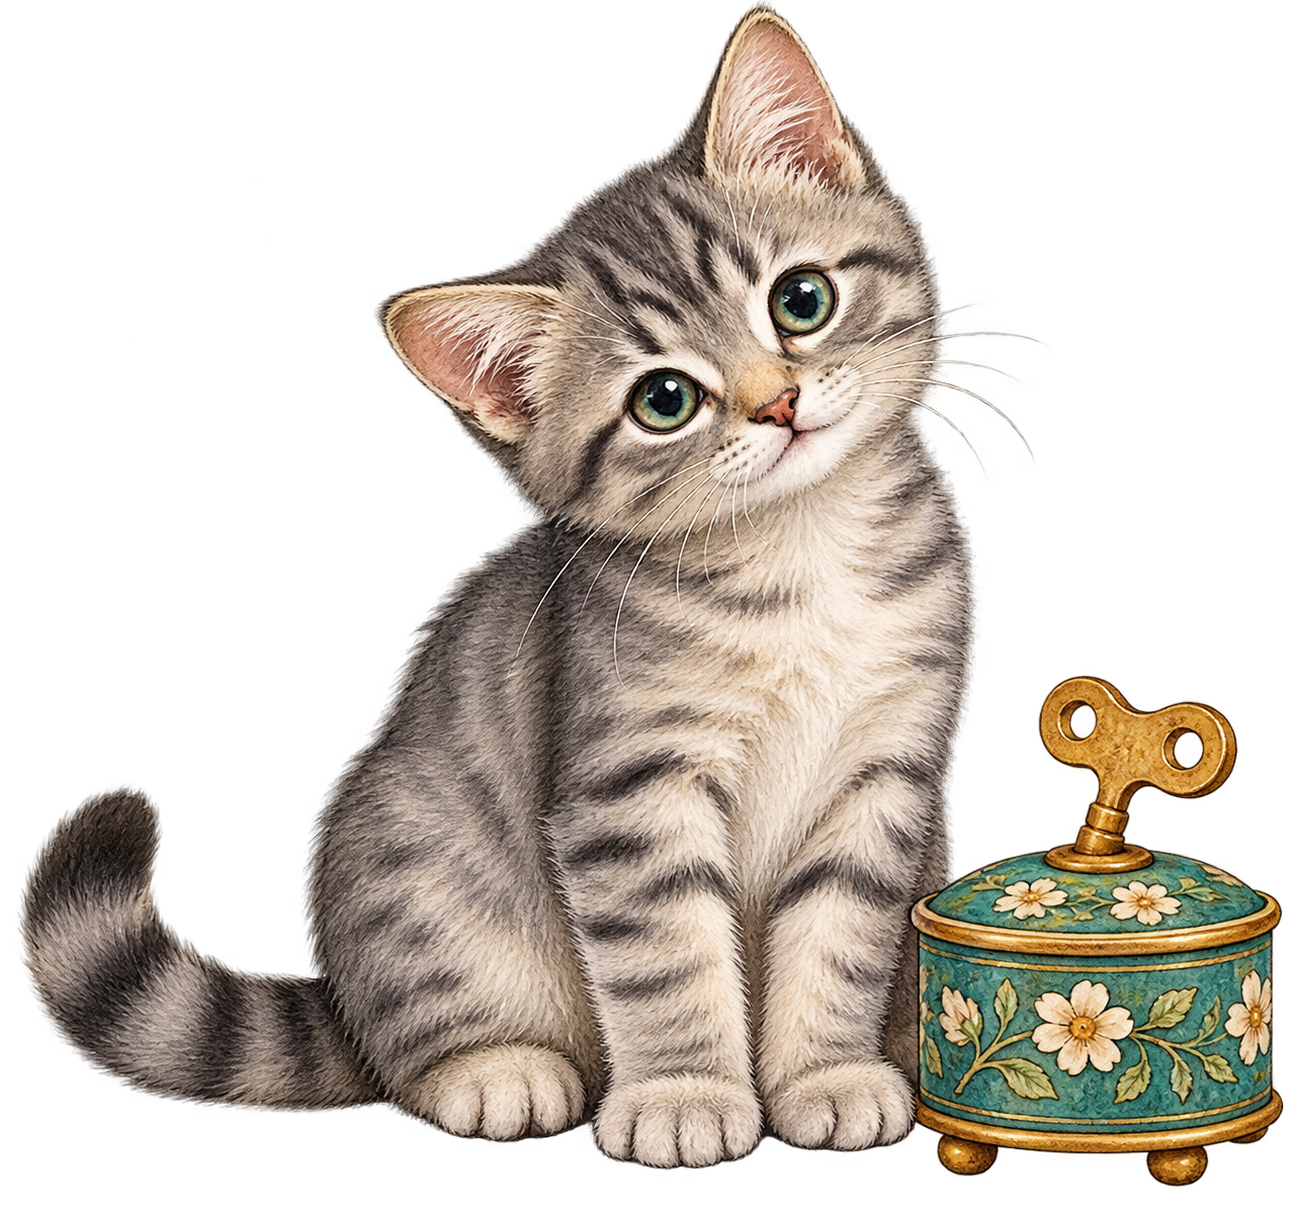
\includegraphics[width=54mm,height=58mm,keepaspectratio]{images/unique/art-94.png}
\label{catflow:94}
\end{wrapfigure}
\textit{Доказательство.} Пусть \(\alpha=\arcsin t\); тогда \(\alpha\in[-\frac\pi2;\frac\pi2]\) и \(\sin\alpha=t\). Угол \(\beta=\frac\pi2-\alpha\) принадлежит \([0;\pi]\), а \(\cos\beta=\sin\alpha=t\). По единственности угла в определении арккосинуса \(\beta=\arccos t\), откуда следует нужное равенство.\hfill\(\blacksquare\)
\par\WFclear\end{minipage}\end{lrbox}%
\ifdim\dimexpr\ht\CatFlowBox+\dp\CatFlowBox\relax<64mm\dp\CatFlowBox=\dimexpr64mm-\ht\CatFlowBox\relax\fi%
\noindent\usebox{\CatFlowBox}\par\addvspace{5pt}

В некоторых источниках обозначения \(\sin^{-1}t\), \(\cos^{-1}t\), \(\operatorname{tg}^{-1}t\) означают обратные функции. Чтобы не путать их с обратными числами \(\frac1{\sin t}\), \(\frac1{\cos t}\), \(\frac1{\operatorname{tg} t}\), здесь используем только записи \(\arcsin\), \(\arccos\), \(\operatorname{arctg}\).

\section{Котангенс и формулы сложения}
\begin{definition}\term{Котангенс} (\emph{cotangent}) — функция \(\operatorname{ctg}x=\frac{\cos x}{\sin x}\), определённая при \(x\ne\pi k\), \(k\in\mathbb Z\). В англоязычной литературе обычно пишут \(\cot x\).\end{definition}
\par\addvspace{5pt}\begin{lrbox}{\CatFlowBox}\begin{minipage}[t]{\linewidth}
\setlength{\parskip}{5pt}\setlength{\columnsep}{4.5mm}\setlength{\intextsep}{0pt}
\begin{wrapfigure}[12]{r}{54mm}

\includegraphics[width=54mm,height=58mm,keepaspectratio]{images/unique/art-98.png}
\label{catflow:98}
\end{wrapfigure}
Котангенс удобно рассматривать по отдельным промежуткам между соседними точками \(\pi k\). На каждом таком промежутке имеется одна непрерывная ветвь. Сдвиг на \(\pi\) меняет знаки и синуса, и косинуса, поэтому их отношение сохраняется. В прямоугольном треугольнике котангенс острого угла равен отношению прилежащего катета к противолежащему. Запись \(\operatorname{ctg}x=\frac1{\operatorname{tg}x}\) допустима только тогда, когда оба выражения определены: например, при \(x=\frac\pi2\) котангенс равен нулю, а тангенс вообще не определён.
\par\WFclear\end{minipage}\end{lrbox}%
\ifdim\dimexpr\ht\CatFlowBox+\dp\CatFlowBox\relax<64mm\dp\CatFlowBox=\dimexpr64mm-\ht\CatFlowBox\relax\fi%
\noindent\usebox{\CatFlowBox}\par\addvspace{5pt}
\begin{theorem}[Основные свойства котангенса]\label{thm:legacy-c15-2}
Функция \(\operatorname{ctg}\) нечётна и имеет период \(\pi\). Её нули равны \(\frac\pi2+\pi k\). При \(\sin x\ne0\) выполнено \(1+\operatorname{ctg}^2x=\frac1{\sin^2x}\). На \((0;\pi)\) функция строго убывает.
\end{theorem}
\begin{proof}
Первые свойства следуют из знаков, периодичности и нулей синуса и косинуса; тождество получается делением \(\sin^2x+\cos^2x=1\) на \(\sin^2x\). Для \(0<x<y<\pi\) имеем
\[
\operatorname{ctg}x-\operatorname{ctg}y=\frac{\sin(y-x)}{\sin x\sin y}>0.
\]
Здесь использована формула синуса разности, доказанная ниже; все три синуса положительны.
\end{proof}
Для следующего доказательства достаточно двух операций с координатными парами. Направленному отрезку из начала координат в точку \((a,b)\) сопоставляем пару \((a,b)\). Складываем пары покоординатно: \((a,b)+(c,d)=(a+c,b+d)\); геометрически это правило параллелограмма. Умножение на число задаём как \(t(a,b)=(ta,tb)\): длина меняется в \(|t|\) раз, а при \(t<0\) направление меняется на противоположное. Такие пары называют векторами (\emph{vectors}). Поворот вокруг начала переводит параллелограмм в параллелограмм и сохраняет отношения длин на одной прямой, поэтому сохраняет обе операции. Подробная теория векторов дана в главе \ref{chap:c18}.

\begin{theorem}[Формулы сложения и двойного угла]\label{thm:legacy-c15-3}
Для любых действительных \(x,y\)
\[
\begin{aligned}
\sin(x+y)&=\sin x\cos y+\cos x\sin y,\\
\cos(x+y)&=\cos x\cos y-\sin x\sin y.
\end{aligned}
\]
Замена \(y\) на \(-y\) даёт формулы разности; при \(y=x\) получаем \(\sin2x=2\sin x\cos x\), \(\cos2x=\cos^2x-\sin^2x\).
\end{theorem}
\par\addvspace{5pt}\begin{lrbox}{\CatFlowBox}\begin{minipage}[t]{\linewidth}
\setlength{\parskip}{5pt}\setlength{\columnsep}{4.5mm}\setlength{\intextsep}{0pt}
\begin{wrapfigure}[11]{l}{54mm}

\includegraphics[width=54mm,height=58mm,keepaspectratio]{images/unique/art-133.png}
\label{catflow:133}
\end{wrapfigure}
\textit{Доказательство.} При повороте плоскости вокруг нуля на угол \(x\) вектор \((1,0)\) переходит в \((\cos x,\sin x)\), а перпендикулярный ему вектор \((0,1)\) — в \((-\sin x,\cos x)\). Поворот сохраняет сложение векторов и умножение на действительное число: это видно по повороту параллелограмма и направленных отрезков на одной прямой. Поэтому образ \((\cos y,\sin y)\) равен
\[
(\cos x\cos y-\sin x\sin y,\;\sin x\cos y+\cos x\sin y).
\]
Но последовательные повороты на \(y\) и \(x\) дают поворот на \(x+y\). Сравнение координат доказывает обе формулы. Нечётность синуса и чётность косинуса дают разность; подстановка \(y=x\) — двойной угол.\hfill\(\blacksquare\)
\par\WFclear\end{minipage}\end{lrbox}%
\ifdim\dimexpr\ht\CatFlowBox+\dp\CatFlowBox\relax<64mm\dp\CatFlowBox=\dimexpr64mm-\ht\CatFlowBox\relax\fi%
\noindent\usebox{\CatFlowBox}\par\addvspace{5pt}

\begin{theorem}[Сложение тангенсов]\label{thm:legacy-c15-4}
Если \(\cos x\ne0\), \(\cos y\ne0\), \(\cos(x+y)\ne0\), то
\[
\operatorname{tg}(x+y)=\frac{\operatorname{tg}x+\operatorname{tg}y}{1-\operatorname{tg}x\operatorname{tg}y}.
\]
\end{theorem}
\begin{proof}Разделим формулы сложения синуса и косинуса друг на друга, а затем числитель и знаменатель на \(\cos x\cos y\). Последний знаменатель равен \(\frac{\cos(x+y)}{\cos x\cos y}\ne0\).\end{proof}

\par\noindent\begin{minipage}{\linewidth}\section*{Графики}
\begin{center}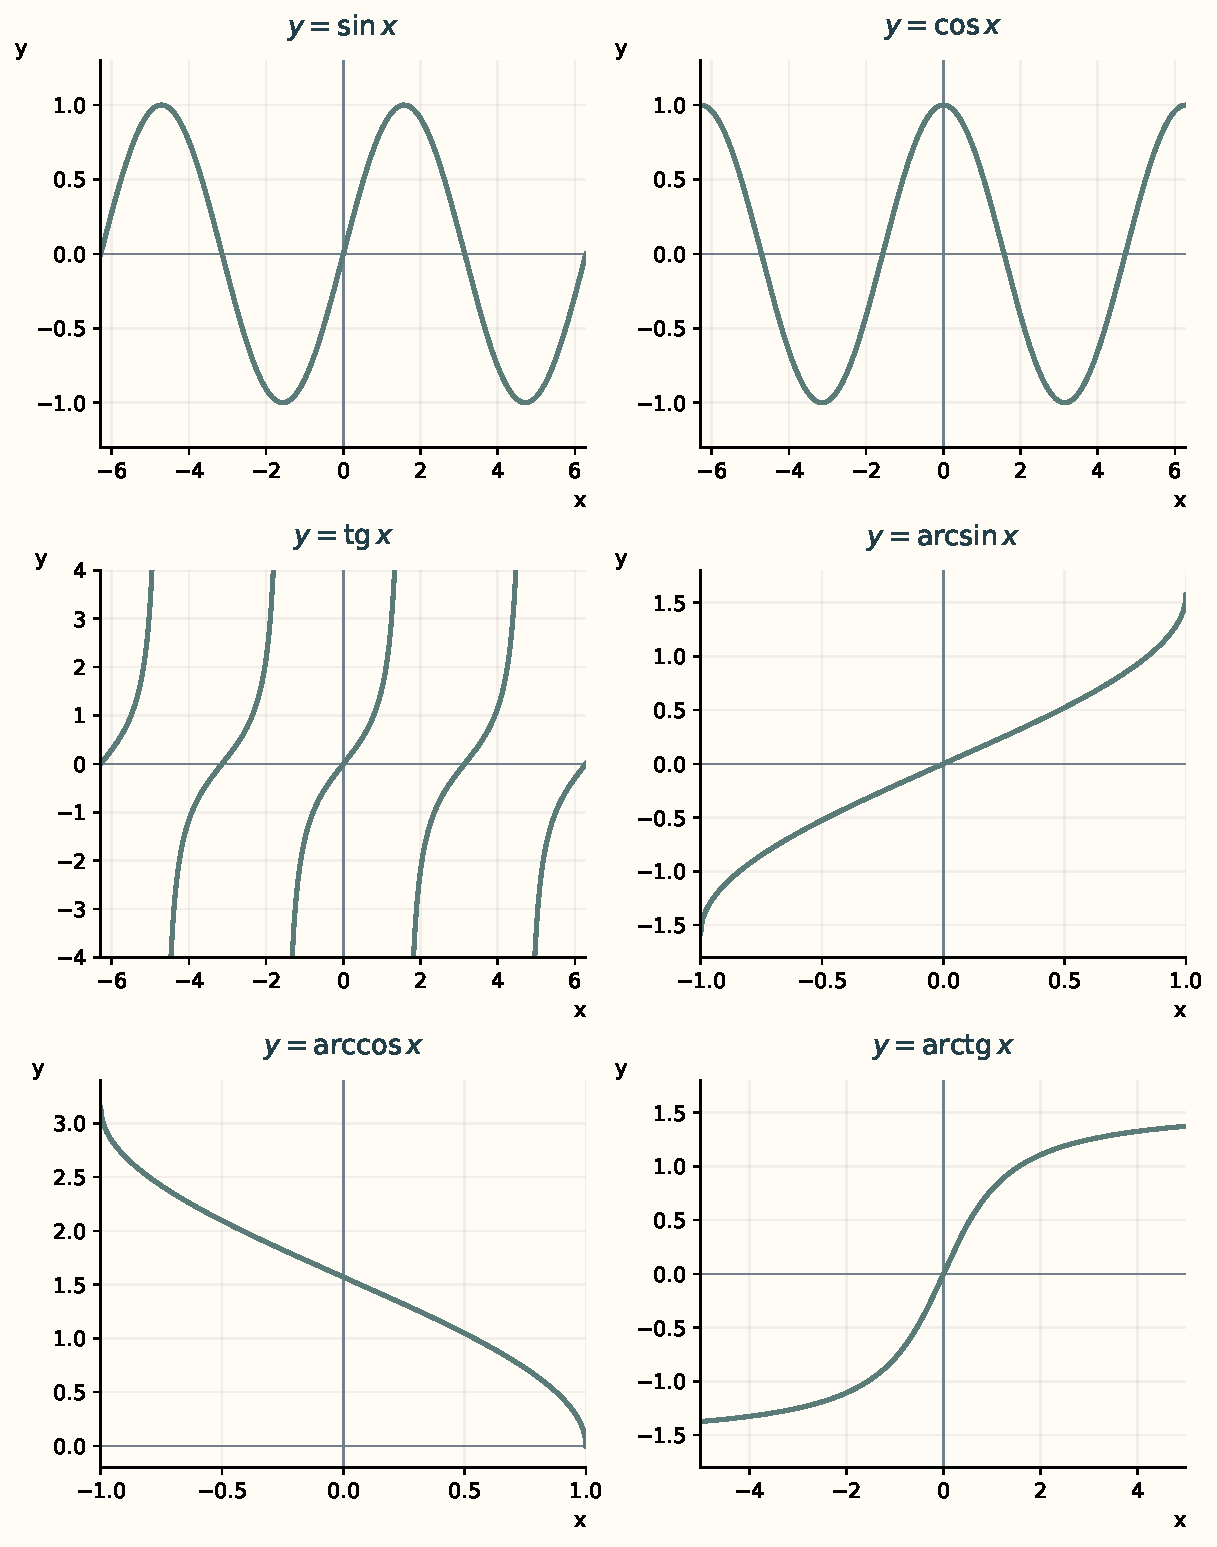
\includegraphics[width=\textwidth,height=.79\textheight,keepaspectratio]{images/atlas-trigonometry.pdf}\par\small Тригонометрические и обратные функции\end{center}\end{minipage}\par
\par\noindent\begin{minipage}{\linewidth}\section*{Тангенс на большом промежутке}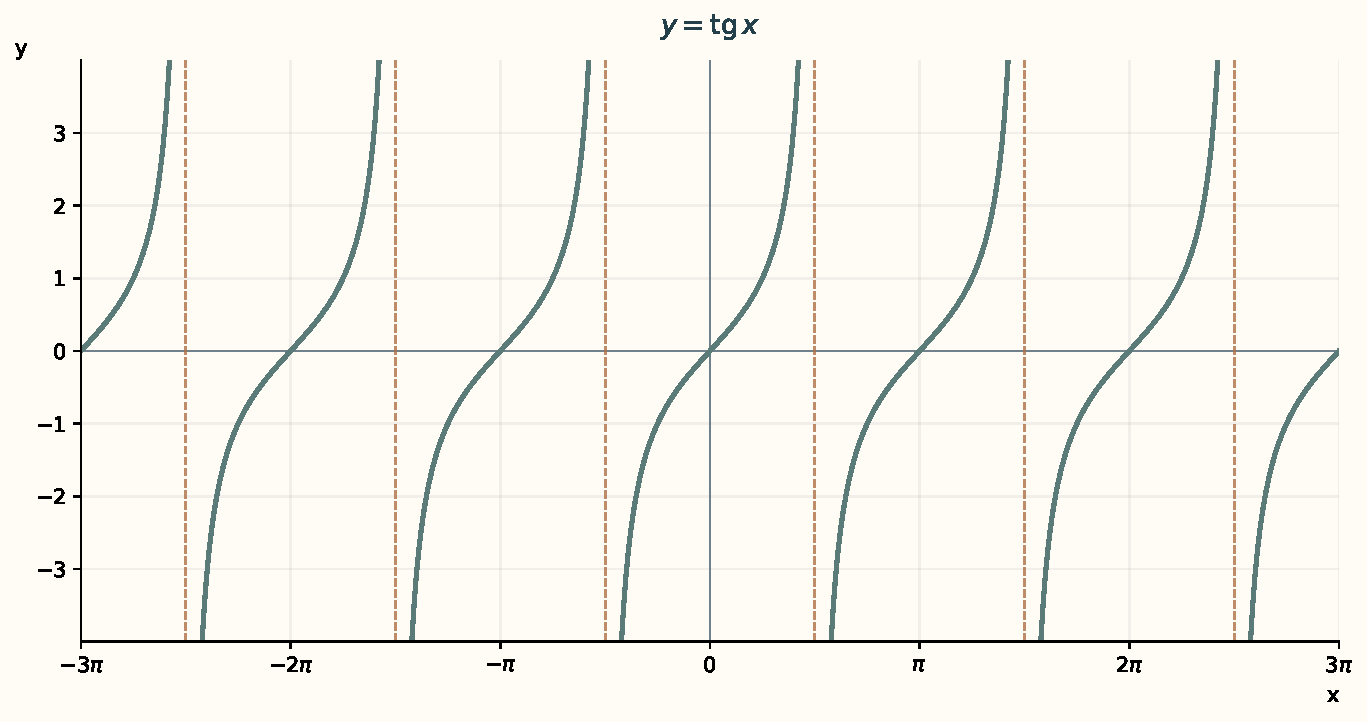
\includegraphics[width=\linewidth]{images/graph-tangent.pdf}\par Пунктиром отмечены прямые \(x=\frac\pi2+\pi k\), \(k\in\mathbb Z\), где тангенс не определён. Соседние ветви повторяются с периодом \(\pi\); через разрывы график не соединяется.\end{minipage}\par
\par\noindent\begin{minipage}{\linewidth}\section*{Котангенс на большом промежутке}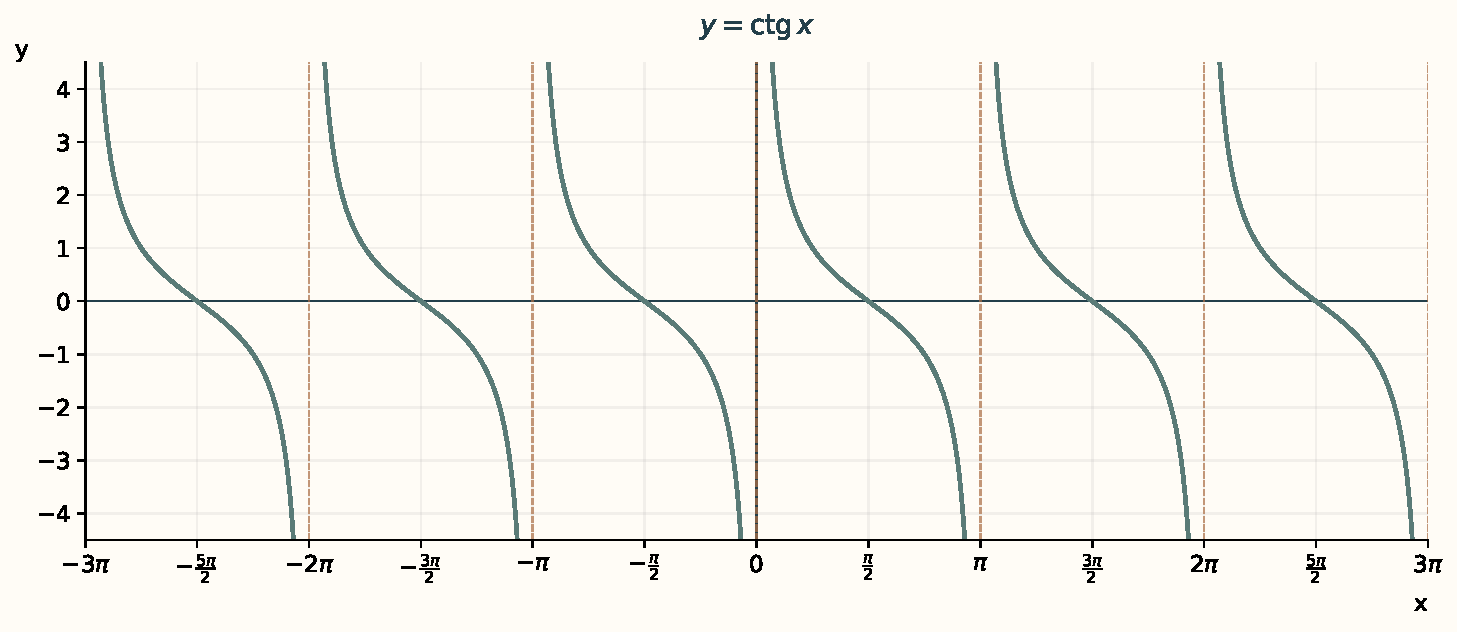
\includegraphics[width=\linewidth]{images/graph-cotangent.pdf}\par Пунктирные прямые \(x=\pi k\), \(k\in\mathbb Z\), не входят в область определения. Каждая ветвь строго убывает; период равен \(\pi\).\end{minipage}\par
\Needspace{7\baselineskip}\section*{Задачи}
\begingroup\setlength{\parskip}{2pt}
\noindent\begin{minipage}[t]{\linewidth}\textbf{24.1.} Переведи \(30 {}^{\circ},\allowbreak 90 {}^{\circ}\) и \(150 {}^{\circ}\) в радианы.\par\end{minipage}\par
\noindent\begin{minipage}[t]{\linewidth}\textbf{24.2.} Переведи \(\dfrac{\pi }{4}\) и \(\dfrac{7 \pi }{6}\) в градусы.\par\end{minipage}\par
\noindent\begin{minipage}[t]{\linewidth}\textbf{24.3.} Вычисли \(\sin  (\dfrac{\pi }{6}),\allowbreak \cos  (\dfrac{\pi }{3}),\allowbreak \operatorname{tg}  (\dfrac{\pi }{4})\).\par\end{minipage}\par
\noindent\begin{minipage}[t]{\linewidth}\textbf{24.4.} Определи знаки \(\sin \) и \(\cos \) для угла \(\dfrac{5 \pi }{6}\).\par\end{minipage}\par
\noindent\begin{minipage}[t]{\linewidth}\textbf{24.5.} Найди \(\sin  (- \dfrac{\pi }{6})\) и \(\cos  (- \dfrac{\pi }{3})\).\par\end{minipage}\par
\par\addvspace{5pt}\begin{lrbox}{\CatFlowBox}\begin{minipage}[t]{\linewidth}
\setlength{\parskip}{5pt}\setlength{\columnsep}{4.5mm}\setlength{\intextsep}{0pt}
\begin{wrapfigure}[12]{l}{54mm}

\includegraphics[width=54mm,height=58mm,keepaspectratio]{images/unique/art-27.png}
\label{catflow:27}
\end{wrapfigure}
\textbf{24.6.} Упрости \(\sin ^{2} x + \cos ^{2} x + 2\).\par

\textbf{24.7.} Если \(\sin  x = \dfrac{3}{5}\) и \(0 < x < \dfrac{\pi }{2}\), найди \(\cos  x\) и \(\operatorname{tg}  x\).\par

\textbf{24.8.} Найди \(\sin  (\pi  - x)\) и \(\cos  (\pi  - x)\) через функции \(x\).\par

\textbf{24.9.} Реши \(\sin  x = 0\) при \(x \in  [0;\allowbreak 2 \pi ]\).\par

\textbf{24.10.} Реши \(\cos  x = \dfrac{1}{2}\) при \(x \in  [0;\allowbreak 2 \pi ]\).\par

\textbf{24.11.} Построй \(y = \sin  x\) на \([0;\allowbreak 2 \pi ]\). Укажи нули, максимум и минимум.\par

\textbf{24.12.} Найди наименьший положительный период \(y = \sin  (2 x)\).\par
\par\WFclear\end{minipage}\end{lrbox}%
\ifdim\dimexpr\ht\CatFlowBox+\dp\CatFlowBox\relax<64mm\dp\CatFlowBox=\dimexpr64mm-\ht\CatFlowBox\relax\fi%
\noindent\usebox{\CatFlowBox}\par\addvspace{5pt}

\noindent\begin{minipage}[t]{\linewidth}\textbf{24.13.} Солнечный луч образует с землёй угол \(45 {}^{\circ}\). Тень вертикального столба равна \(6\) м. Найди высоту столба.\par\end{minipage}\par
\noindent\begin{minipage}[t]{\linewidth}\textbf{24.14.} Лестница длиной \(10\) м образует с горизонтальной землёй угол \(30 {}^{\circ}\). На какой высоте находится её верх?\par\end{minipage}\par
\noindent\begin{minipage}[t]{\linewidth}\textbf{24.15.} Колесо обозрения радиусом \(10\) м имеет центр на высоте \(12\) м. Высота кабинки \(h = 12 + 10 \sin  \alpha \). Найди высоту при \(\alpha  = 0,\allowbreak \dfrac{\pi }{2}\) и \(\dfrac{3 \pi }{2}\).\par\end{minipage}\par
\noindent\begin{minipage}[t]{\linewidth}\textbf{24.16.}\starmark{} Реши \(2 \sin ^{2} x - 3 \sin  x + 1 = 0\) при \(x \in  [0;\allowbreak 2 \pi ]\).\par\end{minipage}\par
\noindent\begin{minipage}[t]{\linewidth}\textbf{24.17.}\starmark{} Луч образует с землёй угол \(30 {}^{\circ}\). Длина тени вертикального дерева \(12\) м. Найди высоту дерева в точном виде.\par\end{minipage}\par
\noindent\begin{minipage}[t]{\linewidth}\textbf{24.18.}\starmark{} Высота кабинки задана \(h (t) = 15 - 12 \cos  (\dfrac{\pi  t}{20})\) метров, где \(t\) — секунды от начала движения. Найди минимальную и максимальную высоты и время первого достижения максимума при \(t \ge  0\).\begin{center}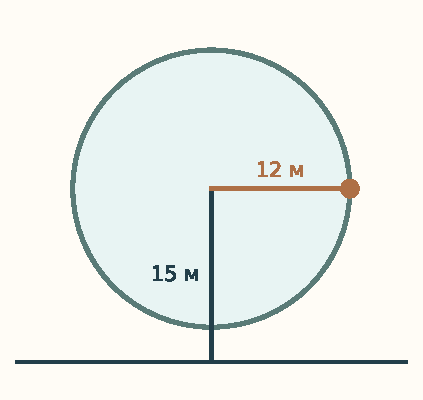
\includegraphics[width=.7\linewidth,height=45mm,keepaspectratio]{images/diagram-wheel.pdf}\end{center}\par\end{minipage}\par
\noindent\begin{minipage}[t]{\linewidth}\textbf{24.19.}\starmark{} Докажи нечётность арксинуса: \(\arcsin(-t)=-\arcsin t\) для \(t\in[-1;1]\). В доказательстве проверь область значений угла, а не только равенство синусов.\par\end{minipage}\par
\noindent\begin{minipage}[t]{\linewidth}\textbf{24.20.}\starmark{} Докажи тождество \(\arccos(-t)=\pi-\arccos t\) при \(t\in[-1;1]\).\par\end{minipage}\par
\noindent\begin{minipage}[t]{\linewidth}\textbf{24.21.} Вычисли \(\arcsin0\), \(\arcsin\dfrac12\), \(\arcsin(-\dfrac{\sqrt3}{2})\).\par\end{minipage}\par
\noindent\begin{minipage}[t]{\linewidth}\textbf{24.22.} Вычисли \(\arccos(-\dfrac12)\), \(\arccos1\), \(\arccos0\).\par\end{minipage}\par
\noindent\begin{minipage}[t]{\linewidth}\textbf{24.23.} Вычисли \(\operatorname{arctg}(-1)\), \(\operatorname{arctg}\sqrt3\), \(\operatorname{arctg}0\).\par\end{minipage}\par
\noindent\begin{minipage}[t]{\linewidth}\textbf{24.24.}\starmark{} Вычисли \(\arcsin(\sin\dfrac{5\pi}6)\), \(\arccos(\cos\dfrac{5\pi}3)\), \(\operatorname{arctg}(\operatorname{tg}\dfrac{3\pi}4)\). Для каждого ответа проверь диапазон обратной функции.\par\end{minipage}\par
\noindent\begin{minipage}[t]{\linewidth}\textbf{24.25.} Найди \(\cos(\arcsin\dfrac35)\) и \(\sin(\arccos(-\dfrac35))\). Обоснуй выбор знака квадратного корня.\par\end{minipage}\par
\noindent\begin{minipage}[t]{\linewidth}\textbf{24.26.} Реши \(\arcsin(2x-1)=\dfrac\pi6\). Сначала найди область допустимых значений.\par\end{minipage}\par
\noindent\begin{minipage}[t]{\linewidth}\textbf{24.27.} Реши \(\operatorname{arctg}(x-2)=-\dfrac\pi4\).\par\end{minipage}\par
\noindent\begin{minipage}[t]{\linewidth}\textbf{24.28.} Построй эскиз \(y=\operatorname{arctg} x\), отметив точки с аргументами \(-1\), \(0\), \(1\). Укажи область определения, область значений и чётность. Может ли значение функции быть равным \(\dfrac\pi2\)?\par\end{minipage}\par
\noindent\begin{minipage}[t]{\linewidth}\textbf{24.29.} Найди \(\operatorname{ctg}\dfrac\pi6\), \(\operatorname{ctg}\dfrac\pi4\), \(\operatorname{ctg}\dfrac\pi3\), \(\operatorname{ctg}\dfrac\pi2\).\par\end{minipage}\par
\noindent\begin{minipage}[t]{\linewidth}\textbf{24.30.} Укажи область определения и нули \(f(x)=\operatorname{ctg}(2x)\).\par\end{minipage}\par
\noindent\begin{minipage}[t]{\linewidth}\textbf{24.31.} Реши \(\operatorname{ctg}x=\sqrt3\).\par\end{minipage}\par
\par\addvspace{5pt}\begin{lrbox}{\CatFlowBox}\begin{minipage}[t]{\linewidth}
\setlength{\parskip}{5pt}\setlength{\columnsep}{4.5mm}\setlength{\intextsep}{0pt}
\begin{wrapfigure}[13]{r}{54mm}

\includegraphics[width=54mm,height=58mm,keepaspectratio]{images/unique/art-134.png}
\label{catflow:134}
\end{wrapfigure}
\textbf{24.32.} В прямоугольном треугольнике катет, прилежащий к острому углу \(\alpha\), равен \(6\) см, противолежащий — \(8\) см. Найди \(\operatorname{ctg}\alpha\) и гипотенузу.\par

\textbf{24.33.} Построй графики \(y=\operatorname{ctg}x\) и \(y=\operatorname{ctg}(x-\dfrac\pi4)\) на нескольких периодах.\par

\textbf{24.34.} Докажи \(\operatorname{tg}x\operatorname{ctg}x=1\). Почему равенство нельзя подставлять при \(x=\dfrac\pi2\)?\par

\textbf{24.35.}\starmark{} Вычисли точно \(\sin\dfrac{5\pi}{12}\) и \(\cos\dfrac{5\pi}{12}\), используя \(\dfrac{5\pi}{12}=\dfrac\pi4+\dfrac\pi6\).\par

\textbf{24.36.}\starmark{} Докажи \(\operatorname{ctg}(x+y)=\dfrac{\operatorname{ctg}x\operatorname{ctg}y-1}{\operatorname{ctg}x+\operatorname{ctg}y}\), явно указав условия.\par
\par\WFclear\end{minipage}\end{lrbox}%
\ifdim\dimexpr\ht\CatFlowBox+\dp\CatFlowBox\relax<64mm\dp\CatFlowBox=\dimexpr64mm-\ht\CatFlowBox\relax\fi%
\noindent\usebox{\CatFlowBox}\par\addvspace{5pt}

\endgroup
